\chapter{Quantum kinetic theory model of a continuous atom laser}
\label{KineticTheory}
\graphicspath{{Figures/KineticTheory/}{Figures/Common/}}

Pumping an atom laser, just like pumping an optical laser, is a necessarily irreversible process. In quantum mechanics, irreversibility enters through the coupling of a system to a large number of modes, known as a reservoir. Although, as quantum mechanics is symmetric under time-reversal, any process can be reversed by an appropriate unitary operation, such an operation can become impractical due to the large number of modes involved making such processes irreversible for all intents and purposes.

There are two choices of reservoir to provide the necessary irreversibility in pumping an atom laser: the electromagnetic and atomic modes. The former was considered in the previous chapter; the latter is the subject of this chapter. The results presented in this chapter have been submitted for publication\footnote{FIXME: Do this.}. The results and analysis presented in \sectionref{KineticTheory:Results} of this chapter was my own work. The model presented in \sectionref{KineticTheory:Model} is based on prior work \citep{Davis:2000vn,Bijlsma:2000}. The derivation of the three-body loss term in \sectionref{KineticTheory:3BodyLoss} and the code the results in this chapter are based on are the work of \emph{Matthew Davis}.

\section{Motivation}

Continuous pumping of an atom laser is a key tool for producing superior atomic sources. Besides the obvious benefit of higher flux, it also promises improved modal stability and linewidth, much as it does for the optical laser.

The two essential steps towards providing a continuous pumping mechanism for an atom laser are the provision of atoms from an external source to the atomic trap, and then a process that causes at least some of those atoms to make an irreversible, atom-stimulated transition into the BEC. Sequential reloading of a FIXME.

This method has the advantage that it can be performed without the presence of resonant light, but the obvious disadvantage that it relies on the system approaching thermal equilibrium, and will therefore be reversed by the addition of atoms above the condensate temperature. In this chapter it is demonstrated that a driven system undergoing evaporative cooling can produce a high-flux, phase-stable atom laser for a range of experimental parameters.

\section{Scheme}

\begin{figure}
    \centering
        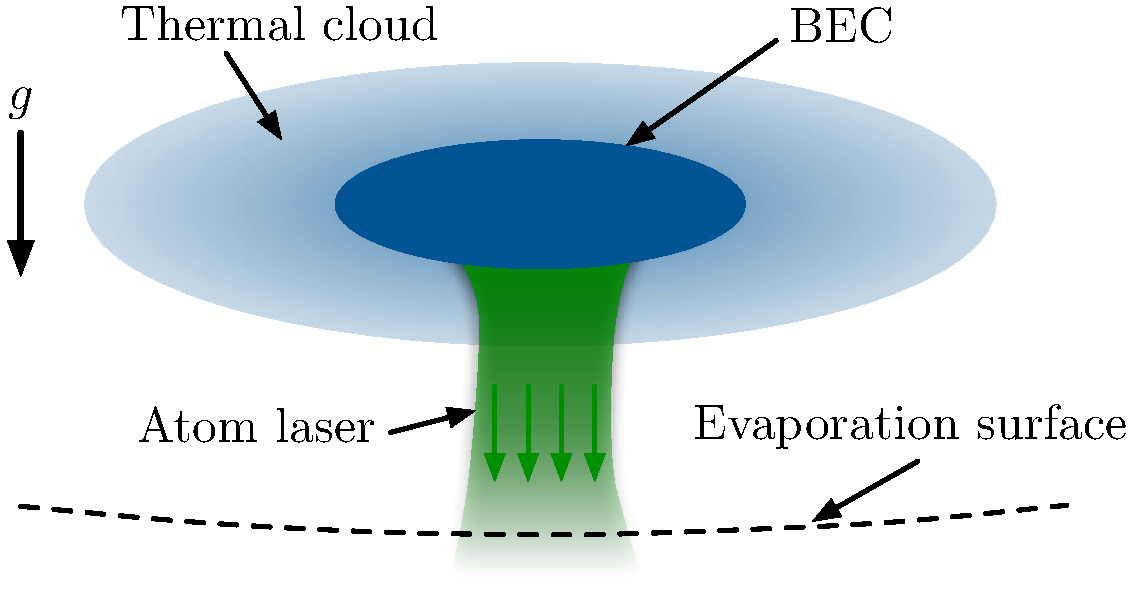
\includegraphics[width=10cm]{QKTScheme}
    \caption{Schematic of the experimental setup}
    \label{KineticTheory:QKTScheme}
\end{figure}


The proposed scheme for a pumped atom laser is illustrated in \figureref{KineticTheory:QKTScheme}, and is conceptually very similar to the evaporative cooling process that is frequently used in the final stage of the production of BEC. 






In order to have net gain into the BEC mode while adding uncondensed atoms to the trap, the system must not be allowed to reach thermal equilibrium. If the thermal vapour is replenished from a source and the radio frequency `scalpel' that produces the forced evaporation is tuned so that atoms of energy $E_c$ and higher are rapidly and continually removed from the trap, then the condensate will continually experience gain and loss as though it was in the middle of an evaporative step. As $E_c$ is lowered, a larger fraction of the scattering processes that leave atoms in the condensate mode become irreversible. This suggests that there must be some value of $E_c$ for which the condensate experiences net gain. What is not clear is whether the net gain can proceed efficiently, i.e. on a timescale much shorter than other losses from the condensate. Lowering $E_c$ also reduces the total number of thermal atoms present. In the limit that $E_c$ reaches the condensate energy, there will be no background gas at all, and the condensate cannot experience net gain. We therefore expect that for a given set of parameters, there will be an optimal value for $E_c$ that maximises the net gain, which may or may not be positive. In order to examine this issue, we have employed quantum kinetic theory (QKT), which has been effective in describing the growth of condensates \citep{Davis:2000vn,Bijlsma:2000}.

\section{Quantum Kinetic Theory Model}
\label{KineticTheory:Model}
In the model section we will describe the equations and state them. There will be no derivation, with the exception of the three-body loss terms. The equations are derived in sufficient detail in \citep{Bijlsma:2000}. Code, and three-body loss terms derivation performed by \emph{Matthew Davis}.

\subsection{Derivation of the three-body loss term}
\label{KineticTheory:3BodyLoss}

\section{Results}
\label{KineticTheory:Results}
This is my contribution. Example simulations demonstrating time-dependence of the distributions, the dependence on $\eta$. Behaviour (and simple model) in the absence of three-body loss and why this is both obvious and unrealistic. Behaviour (and simple model in high-temperature limit) in the presence of three-body loss.

Joe has suggested that we not rely on the high-temperature limit, but I would really, really like to have that in.

\section{Conclusion}
Thermal sources must be close to degenerate to be useful. 